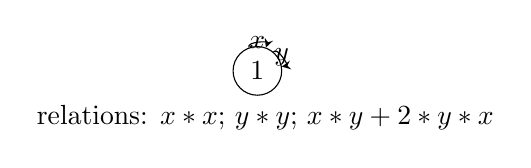
\begin{tikzpicture}[>=stealth]
  \node[draw, circle] (v1) at (0, 0) {$1$};
  \draw[->] (v1) to[loop, in=70, out=110] node {$x$} (v1);
  \draw[->] (v1) to[loop, in=10, out=50] node {$y$} (v1);
  \node[align=left, below] at (current bounding box.south) {relations: $x*x$;  $y*y$;  $x*y + 2*y*x$};
\end{tikzpicture}
